\documentclass{article}
\usepackage[utf8]{inputenc}
\usepackage{amsmath,amssymb}
\usepackage{cancel}
\usepackage{makecell}
\usepackage[a4paper, total={6in, 9in}]{geometry}
\usepackage{authblk}
\usepackage{graphicx}
\graphicspath{{.}}
\author{Zihan Zhao}
\affil{1001103708}
\title{Homework 4}
\date{}
\begin{document}
\maketitle
\renewcommand{\thesubsection}{(\alph{subsection})}
\section{Multilayer Perceptron}
There are 2 units on input layer, 6 units on hidden layer and 2 units on output layer. The $W,b$ for each layer edges are as following:
\begin{align*}
    W^{(1)} &= 
    \begin{bmatrix}
        1 & -1\\
        -1 & 1\\
        1 & 0\\
        0 & 1\\
        -1 & 0\\
        0 & -1\\
    \end{bmatrix}
    b^{(1)} = 
    \begin{bmatrix}
        0\\
        0\\
        0\\
        0\\
        0\\
        0\\
    \end{bmatrix}\\
    W^{(2)} &= 
    \begin{bmatrix}
        -\frac{1}{2} & -\frac{1}{2} & \frac{1}{2} & \frac{1}{2} & -\frac{1}{2} & -\frac{1}{2}\\
        \frac{1}{2} & \frac{1}{2} & \frac{1}{2} & \frac{1}{2} & -\frac{1}{2} & -\frac{1}{2}\\
    \end{bmatrix}
    b^{(2)} = 
    \begin{bmatrix}
        0\\
        0\\
    \end{bmatrix}\\
\end{align*}
How does it work?\\
\begin{align*}
h1&=ReLU(x_1-x_2)\\
h2&=ReLU(x_2-x_1)\\
h3&=ReLU(x_1)\\
h4&=ReLU(x_2)\\
h5&=ReLU(-x_1)\\
h6&=ReLU(-x_2)\\
\intertext{We can get $y_1$, $y_2$}
y1&=-\frac{1}{2}h1 + -\frac{1}{2}h2 + \frac{1}{2}h3 + \frac{1}{2}h4 + -\frac{1}{2}h5 + -\frac{1}{2}h6\\
&=-\frac{1}{2}h1 + -\frac{1}{2}h2 + \frac{1}{2}(h3-h5) + \frac{1}{2}(h4-h6)\\
&=-\frac{1}{2}h1 + -\frac{1}{2}h2 + \frac{1}{2}(max(0,x_1)-max(0,-x_1)) + \frac{1}{2}(max(0,x_2)-max(0,-x_2))\\
\intertext{If $x_1 \geq 0$, $max(0,x_1)-max(0,-x_1)=x_1-0=x_1$;}
\intertext{If $x_1 < 0$, $max(0,x_1)-max(0,-x_1)=0-(-x_1)=x_1$; So is $x_2$. Then,}\\
y1&=-\frac{1}{2}h1 + -\frac{1}{2}h2 + \frac{1}{2}x_1+\frac{1}{2}x_2\\
y2&=\frac{1}{2}h1 + \frac{1}{2}h2 + + \frac{1}{2}x_1+\frac{1}{2}x_2\\
\intertext{If $x_1 \geq x_2$,}
h1&=x_1-x_2\\
h2&=0\\
\intertext{Then,}
y1&=-\frac{1}{2}(x_1-x_2) + -\frac{1}{2}*0 + \frac{1}{2}x_1+\frac{1}{2}x_2\\
&=-\frac{1}{2}x_1+ -\frac{1}{2}(-x_2) + \frac{1}{2}x_1+\frac{1}{2}x_2\\
&=x_2\\
y2&=\frac{1}{2}(x_1-x_2) + \frac{1}{2}*0 + \frac{1}{2}x_1+\frac{1}{2}x_2\\
&=x_1\\
\intertext{If $x_1 < x_2$,}
h1&=0\\
h2&=x_2-x_1\\
\intertext{Then,}
y1&=-\frac{1}{2}(x_2-x_1) + \frac{1}{2}x_1+\frac{1}{2}x_2\\
&=x_1\\
y2&=\frac{1}{2}(x_2-x_1) + \frac{1}{2}x_1+\frac{1}{2}x_2\\
&=x_2\\
\intertext{They are sorted in order.}
\end{align*}
\section{Backprop}
\subsection{}
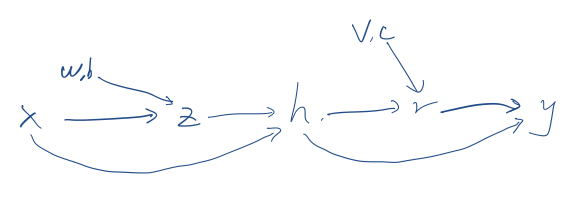
\includegraphics[width=\textwidth,height=\textheight,keepaspectratio]{cg.png}
\subsection{}
Assume we know $\overline{y} = \frac{\partial L}{\partial y} $, 
\begin{align*}
    \frac{\partial L}{\partial V} &= \overline{y}\frac{\partial y}{\partial V}\\
    &= \overline{y}\frac{\partial \phi (r)}{\partial V}+\overline{y}\frac{\partial h}{\partial V}\\
    &= \overline{y}\phi ^\prime (r)\frac{\partial Vh+c}{\partial V}+0\\
    &= \overline{y}\phi ^\prime (r)h\\
    \frac{\partial L}{\partial c} &= \overline{y}\frac{\partial y}{\partial c}\\
    &= \overline{y}\frac{\partial \phi (r)}{\partial c}+\overline{y}\frac{\partial h}{\partial c}\\
    &= \overline{y}\phi ^\prime (r)\frac{\partial Vh+c}{\partial c}+0\\
    &= \overline{y}\phi ^\prime (r)\\
    \frac{\partial L}{\partial W} &= \overline{y}\frac{\partial y}{\partial W}\\
    &= \overline{y}\frac{\partial \phi (r)}{\partial W}+\overline{y}\frac{\partial h}{\partial W}\\
    &= \overline{y}\phi ^\prime (r)\frac{\partial Vh+c}{\partial W}+\overline{y}\frac{\partial \phi (z) + x}{\partial W}\\
    &= \overline{y}\phi ^\prime (r)\frac{\partial Vh}{\partial W}+\overline{y}\phi ^\prime (z)\frac{\partial Wx+b}{\partial W}\\
    &= \overline{y}\phi ^\prime (r)V\frac{\partial \phi (z)+x}{\partial W}+\overline{y}\phi ^\prime (z)x\\
    &= \overline{y}\phi ^\prime (r)V\phi ^\prime (z)\frac{\partial Wx+b}{\partial W}+\overline{y}\phi ^\prime (z)x\\
    &= \overline{y}\phi ^\prime (r)V\phi ^\prime (z)x+\overline{y}\phi ^\prime (z)x\\
    \frac{\partial L}{\partial b} &= \overline{y}\frac{\partial y}{\partial b}\\
    &= \overline{y}\frac{\partial \phi (r)}{\partial b}+\overline{y}\frac{\partial h}{\partial b}\\
    &= \overline{y}\phi ^\prime (r)\frac{\partial Vh+c}{\partial b}+\overline{y}\frac{\partial \phi (z) + x}{\partial b}\\
    &= \overline{y}\phi ^\prime (r)\frac{\partial Vh}{\partial b}+\overline{y}\phi ^\prime (z)\frac{\partial Wx+b}{\partial b}\\
    &= \overline{y}\phi ^\prime (r)V\frac{\partial \phi (z)+x}{\partial b}+\overline{y}\phi ^\prime (z)\\
    &= \overline{y}\phi ^\prime (r)V\phi ^\prime (z)\frac{\partial Wx+b}{\partial b}+\overline{y}\phi ^\prime (z)\\
    &= \overline{y}\phi ^\prime (r)V\phi ^\prime (z)+\overline{y}\phi ^\prime (z)\\
\end{align*}
\section{EM for Probabilistic PCA}
\subsection{}
See appendix equations of $p(z)$ and $p(x|z)$,
In this problem, we know $p(z)=N(z|0,1)$ and $p(x|z) = N(x|zu,\sigma ^2I)$. Plug into the equations in appendix. We got:
\begin{align*}
    \mu  &= 0\\
    \varSigma &= 1\\
    A &= u\\
    b &= 0\\
    S &= \sigma ^2I\\
\intertext{Then:}
    C &= (1+u^T(\sigma ^2I)^{-1}u)^{-1}\\
    &= (1+\frac{1}{\sigma ^2}u^Tu)^{-1}\\
    &= \frac{\sigma ^2}{\sigma ^2 + u^Tu}\\
\intertext{Then:}
    mean = m &= C(A^TS^{-1}(x-b)+\varSigma^{-1}\mu)\\
    &= \frac{\sigma ^2}{\sigma ^2 + u^Tu}(u^T\sigma ^{-2}Ix)\\
    &= \frac{u^Tx}{\sigma ^2 + u^Tu}\\
    Var = C &= \frac{\sigma ^2}{\sigma ^2 + u^Tu}\\
\intertext{Then:}
    s = Var + m^2 &=\frac{\sigma ^2}{\sigma ^2 + u^Tu} + \frac{(u^Tx)^2}{(\sigma ^2 + u^Tu)^2}\\
    &=\frac{\sigma ^2(\sigma ^2 + u^Tu)+(u^Tx)^2}{(\sigma ^2 + u^Tu)^2}\\
    &=\frac{\sigma ^4+\sigma ^2u^Tu+(u^Tx)^2}{(\sigma ^2 + u^Tu)^2}\\
\intertext{To conclude:}
    m &= \frac{u^Tx}{\sigma ^2 + u^Tu}\\
    s &=\frac{\sigma ^4+\sigma ^2u^Tu+(u^Tx)^2}{(\sigma ^2 + u^Tu)^2}\\
\end{align*}
\subsection{}
% Find $p(x)$ first using appendix:
% \begin{align*}
%     mean = A\mu + b &= 0\\
%     Cov = A \varSigma A^T+S &= u u^T + \sigma ^2I\\
% \intertext{Then:}
%     p(x) &= \frac{1}{\sqrt{((2\pi )^d(Cov) ^{2d})}}exp()\\
% \end{align*}
Assume the dimension of $x^{(i)}$ is dx1. Find $logp(z,x)$ first:
\begin{align*}
    log(p(z,x)) &= log(p(x|z))+log(p(z))\\
    &= -\frac{\frac{1}{\sigma ^2}(x-zu)^T(x-zu)}{2}log(\frac{1}{\sqrt{((2\pi )^d\sigma ^{2d})}}) + const\\
    &= \frac{\frac{1}{\sigma ^2}(x-zu)^T(x-zu)}{2}log(\sqrt{((2\pi )^d\sigma ^{2d})}) + const\\
    &= \frac{\frac{1}{\sigma ^2}(x-zu)^T(x-zu)}{4}log((2\pi )^d\sigma ^{2d}) + const\\
\intertext{Define a const $D = \frac{log((2\pi )^d\sigma ^{2d})}{4\sigma ^2}$}
    &=D(x-zu)^T(x-zu) + const\\
    &=D(x^Tx-x^Tzu-zu^Tx+zu^Tzu) + const\\
    &=D(-2zu^Tx+z^2u^Tu) + const^\prime\\
\intertext{Then:}
    E[log(p(z,x))] &= -2DE[z]u^Tx + DE[z^2]u^Tu + const^\prime\\
                 &= -2Dmu^Tx + Dsu^Tu + const^\prime\\
\intertext{Drop $const^\prime$, then the constant-dropped expected log-likelihood $L$ is:}
    L &= \frac{1}{N}\sum_{i = 1}^{N}(-2Dm^{(i)}u^Tx^{(i)} + Ds^{(i)}u^Tu)\\
    \frac{\partial L}{\partial u} &= \frac{1}{N}\sum_{i = 1}^{N}(-2Dm^{(i)}x^{(i)} + 2Ds^{(i)}u)\\
\intertext{Let $\frac{\partial L}{\partial u} = 0$, then:}
    \frac{1}{N}\sum_{i = 1}^{N}(-2Dm^{(i)}x^{(i)} + 2Ds^{(i)}u) &= 0\\
    u_{new} &= \frac{\sum_{i = 1}^{N}(m^{(i)}x^{(i)})}{\sum_{i = 1}^{N}s^{(i)}}\\
\end{align*}
\end{document}
